\chapter{Referêncial Teórico}

É apresentado nesse capítulo um conjunto de definições relevantes para o tema dessa proposta de trabalho. Foi realizada uma pesquisa sistemática para selecionar os principais tópicos apoiam o entendimento deste trabalho. Os detalhes estão descritos nas próximas seções.

\section{Teste de Software}

Teste de software é o processo que realiza a avaliação do sistema ou de seus componentes com o objetivo de desvendar o comportamento para garantir que os seus requisitos estão de acordo com o esperado ou não. Em outras palavras teste é execução do sistema, a fim de identificar eventuais lacunas, erros ou requisitos que não foram implementados de acordo com as necessidades requeridas \cite{tutorialsPoint}. Segundo \cite{ansiieee1059}, Teste pode ser definido como o processo de análise do software para detectar as diferenças entre condições existentes e necessárias e avaliar as características do software.

Um bom teste pode ser aquele que tem alta probabilidade de encontrar erros que ainda não foram expostos e um teste bem sucedido é aquele que revela um erro ainda não-descoberto. O teste pode ser manual, automatizado, ou ainda a combinação de ambos \cite{Pressman2002}. A redução de custo, tempo e retrabalho são proporcionais ao quão cedo o processo de testes for iniciado \cite{tutorialsPoint}.

\section{Tipos de Teste de software}

Testes de software podem ser divididos em duas categorias, testes manuais e automatizados.

\subsection{Testes Manuais}

		Este tipo de teste é feito pela execução manual do software, ou seja, sem o uso de qualquer ferramenta automatizada ou qualquer script. O testador assume o papel do usuário final para realizar os testes e identificar qualquer comportamento que não seja esperado ou revelar defeitos. Costumam usar planos de teste, casos de teste e/ou cenários para garantir a integridade dos testes. Também pode ser incluso dentro deste tipo os testes exploratórios, no qual o testador irá explorar o software com o intuito de encontrar erros\cite{tutorialsPoint}.
		
\subsection{Testes Automatizados}

Testes automatizados podem ser definidos como automação de atividades de teste de software, incluindo o desenvolvimento e execução de scripts de testes, verificação de requisitos, como também a utilização de ferramentas de teste automatizadas \cite{Dustin1999}.
 
Entre as razões para o uso da automação dos testes de software podemos citar, por exemplo, executar testes manuais é mais demorado, uso da automação de testes aumenta a  eficiência processo, em um fatia particular temos os testes de regressão, onde os casos de testes são executados de forma iterativa, depois de alterações no software \cite{Dustin1999}.
		
\section{Níveis de testes de Software}

Em \cite{Pressman2002} aponta que a realização de testes apenas quando o sistema está construído é uma abordagem ineficaz. Segundo o autor, a estratégia de testes de software de possuir uma abordagem incremental, começando com os testes de unidades, seguindo com os testes de integração, culminando com os testes do sistema final e ainda acoplando testes que se enquadrem em testes de aceitação.

\subsection{Testes Funcionais}

Este tipo de teste é baseado nas especificações do software que será testado, a aplicação será testada através do fornecimento de entradas e em seguida, os resultados serão examinados para garantir a conformidade com os requisitos de tal funcionalidade \cite{tutorialsPoint}. Basicamente testar se os componentes e o sistema estão feitos, uma atividade ou uma função especifica do código está coerente com o esperado. Neste nível de teste perguntas como "O usuário poderá fazer isso?" ou "Esta função em particular funciona?" podem ser validadas tipicamente através de especificações de requisitos ou funcional \cite{Leung1990}. 

\subsection{Testes Unitários}

É a menor parte que pode ser testada do código que compõe o software, são de granulação fina, comportamento extremamente rápido, por exemplo, métodos de uma classe, uma classe ou classes que podem estar relacionadas. Não verificam o comportamento de unidades integradas com outros serviços ou dependências, garantem que sua função como unidade estão funcionando. Seu objetivo é isolar parte do programa e mostrar que partes individuais estão corretas em termos de requisitos e funcionalidades \cite{James2012}.  Existe um limite para cenários e dados que podem ser aplicados ao nível de testes de unidade, quando é nítido esse esgotamento é necessário o mistura com outras unidades do código e diferentes tipos de testes \cite{tutorialsPoint}.

\subsection{Testes de Integração}

Neste caso, é realizada a combinação de partes da aplicação que serão agrupadas para determinar se funcionamento desse conjunto está trabalhando corretamente \cite{tutorialsPoint}. Alguns defeitos não podem ser encontrados a nível unitário, mas são revelados através da integração com núcleos específicos \cite{Pachawan2014}.

\subsection{Teste de Sistema}

Após a realização dos testes de integração, uma vezes que todos os componentes foram integrados, os testes do sistema como um todo são agora efetuados para garantir que a aplicação atende aos padrões de qualidade desejado \cite{tutorialsPoint}. A aplicação é testada minuciosamente para validar especificações funcionais e técnicas, é construído um ambiente o mais próximo possível do ambiente de produção, para que os testes sejam executados em um ambiente que corresponda ao ambiente no qual o sistema será implantado. O teste do sistema nos retornará a validação dos requisitos de negócio e da arquitetura como todo da aplicação.

\subsection{Teste de Regressão}

Significa testar uma aplicação após o seu código fonte ter sido modificado para validar se ainda continua funcionando devidamente. Consiste em reexecutar casos de testes existentes e verificar se alterações de código não interfere em funcionalidades que estavam trabalhando corretamente, se foram inseridos novos erros ou causa problemas em erros que já foram reparados \cite{Leung1990}. Afim de identificar defeitos introduzidos por novas funcionalidades ou correção de defeitos.

\subsection{Testes de Aceitação}

Nível mais alto que trata da aplicação como uma caixa preta, sem dúvidas considerado um dos mais importantes entre os outros, este tipo de teste é feito na grande parte  pelo time de garantia da qualidade \cite{James2012}. Onde todo time verificará se o produto preenche as especificações solicitadas e satisfaz os requisitos dos clientes. O time responsável terá um conjunto de cenários previamente escritos e que serão usados no momento da validação. Durante a fase de validação outros cenários podem  surgir para aumentar a cobertura dos testes. Testes de aceitação não são apenas para identificação de erros de interfaces, mas também para encontrar divergências que poderão resultar em quebra ou erros graves do sistema \cite{tutorialsPoint}. Para a execução de desse tipo de testes é necessário definir critérios de aceitação a partir dos requisitos do software, estabelecendo como o teste será conduzido e a partir desses critérios, avaliar se o produto satisfaz aos requisitos \cite{SoftexRecife}.

\subsection{Testes Não-Funcionais}

Requisitos não funcionais são declarações que define as qualidades globais ou atributos a serem atendidos pelo sistema resultante \cite{Kirner1996}. Estes requisitos, ao contrário dos requisitos funcionais, não expressão nenhuma função a ser realizada pelo software, e sim comportamentos e restrições que este software deve satisfazer \cite{Cysneiros1997}. Os testes desses requisitos são normalmente executados com ajuda de ferramentas especializadas, com grande planejamento, avaliação arquitetural, aplicando técnicas avançadas \cite{tutorialsPoint}.

Alguns dos considerados mais importantes tipos de validação não funcionais são \cite{tutorialsPoint}:
\begin{itemize}
	\item Teste de Performance
	\item Teste de Carga
	\item Teste de Stress
	\item Teste de Segurança
	\item Teste de Usabilidade
	\item Teste de Portabilidade
\end{itemize}

\section{Automação de testes}

Ainda que a atividade seja complexa, o teste de software nem sempre é realizado de forma sistemática devido a diversos fatores dos projetos, como: tempo e recursos limitados, qualificação do time e dos envolvidos, complexidade e da rapidez da evolução dos sistemas. Sendo assim, a automação de testes uma importante medida para melhorar a eficiência dessas atividades \cite{Fantinato2004}.

Automação de testes é uso de um software para controlar a execução das atividades de teste de um sistema, a comparação dos resultados esperados com os resultados reais, a configuração das pré-condições de teste e outras funções de controle e relatório de teste \cite{Hooda2012}. Atualmente essa prática vem sendo difundida em processos ágeis, como também em Extreme Programmaing (XP), e até mesmo em organizações que ainda utilizam metodologias tradicionais como Rational Unified Process \cite{Lima2012}.

Segundo Fewster e Graham \cite{Fewster1999} afirmam que a automação de testes de software pode reduzir de maneira significativa e impactante o esforço necessário para execução dos testes. Assim como Molinari\cite{Molinari2010}, afirma que testes automatizados aumenta a produtividade e alcança em tempo menor os objetivos do teste. Apesar do grande poder que os testes automatizados apresentam, algumas empresas ainda resistem na aplicação de estratégias de automação de testes, sobretudo, por conta do esforço necessário para iniciar o processo e por demandar mudança na cultura da organização \cite{Lima2012}. Mais rápido que os testes manuais e menos suscetível a erros, máquinas possuem probabilidade de erro bem menor. Aprimorar e aplicar testes automatizados tem se tornado algo crucial nas empresas atualmente, segundo pesquisa realizada em 2008 pelo Forrester Research Inc.

A seguir serão citados e comentados algumas vantagens e dificuldades na implantação de testes automatizados.

\subsection{Vantagens da automação de testes}

De acordo com Fewster e Graham \cite{Fewster1999}, os principais benefícios da automação de testes de software são:

\begin{itemize}
	\item Torna a execução dos testes de regressão mais fácil, tendo em vista a reutilização de casos de testes automatizados de versões antigas em versões seguintes aplicando o esforço manual mínimo em testes manuais.
	\item Permite executar um maior número de testes em menor tempo, aumentando a frequência dos testes e trazendo mais confiança ao sistema;
	\item Execução de testes que seriam inviáveis manualmente falando, como a verificação de cálculos extremamente complexos ou testes de carga com um número alto de acessos;
	\item Aprimorar a utilização dos recursos, permitindo que os testadores reduzam o esforço em atividades repetitivas, conseguindo focar esforços em atividades de planejamento dos testes e na execução de cenários cuja automação é inviável;
	\item Permite aumentar a consistência dos resultados dos testes entre diferentes plataformas, já que as entradas e condições esperadas são as mesmas;
	\item Diminuição do “time to Market”, tendo em vista a redução do tempo do projeto dedicado aos testes;
	\item Aumentar a credibilidade e confiança na qualidade do sistema como um todo, um bom volume de testes automatizados bem planejados e executados com êxito podem trazer para o time um sentimento de confiança na qualidade do produto final.
\end{itemize}

Com base nessas vantagens é possível perceber o grande potencial da automação dos testes na melhoria das atividades que envolvem testes de software. Alguns desses benefícios podem ser evidenciados através da aplicação que será utilizada como caso de estudo desta proposta de trabalho.

\subsection{Desafios da automação de testes}

Em conformidade com Fewster e Graham \cite{Fewster1999} as principais barreiras e desafios na implantação da automação de testes de software em uma organização são:

\begin{itemize}
	\item Expectativas irreais: Automação de testes não é a solução de todos os
problemas e não deve ser vista como tal, deve ser encarada de forma realista;
	\item Prática de testes pobre: Caso o processo de testes adotado pela organização seja ineficaz, com testes mal planejados e documentação inconsistente, é necessário melhorar e corrigir o processo antes da implantação da automação.
	\item Manutenção dos testes: alguns softwares sofrem muitas modificações, o esforço de manutenção dos testes automatizados pode ser maior que o esforço de reexecuta-los manualmente;
	\item Problemas técnicos:  ferramentas de automação de testes também podem sofrer problemas, comprometendo a estratégia de automação. É necessário que haja um responsável  pela automação e tenha conhecimentos técnicos detalhados das ferramentas, para que o sua utilização seja efetiva.
	\item Questões organizacionais: a automação de testes precisa ser implementada na cultura da organização, com alocação de tempo para a escolha de ferramentas e formação, visando entender e selecionar as práticas que melhor se adequam a organização;
\end{itemize}

Diante dessas dificuldades, a implantação de testes automatizados é uma atividade complexa. Deve, dessa forma, ser bem analisada sobre sua necessidade e como deve ser adaptada ao processo atual da organização e time.

\subsection{Técnicas de automação de testes}

As principais técnicas de automação de automação de teste, presentes na literatura são: record and playback, scripts, data-driven e keyword-drivers. Essas técnicas serão expostas a seguir \cite{Fantinato2004}.

\begin{itemize}

	\item Record and playback 
	
Essa técnica se baseia na gravação das ações do usuário durante a interação com a interface gráfica do sistema, convertendo essas ações em scripts de testes que podem ser reproduzidos várias vezes for necessário. Para cada caso de teste é gravado um script de teste completo que inclui os dados de teste (dados de entrada e resultados esperados), o procedimento de teste (passo a passo que representa a lógica de execução) e as ações de teste sobre a aplicação.

Mesmo sendo considerada uma técnica simples e prática, sendo uma abordagem para testes executados poucas vezes, apresenta algumas desvantagens para uma grande quantidade de testes automatizados, com alto custo e dificuldade de manutenção, baixa taxa de reutilização, curto tempo de vida e alta sensibilidade a mudanças no software a ser testado e no ambiente
de teste.

	\item Programação de scripts 
	
É uma extensão da técnica record and playback que utilizando a programação e seus recursos para alterar os scripts gravados, permitindo alcançar uma maior quantidade de verificações de resultados esperados. Com o uso desta técnica é possível obter uma maior taxa de reutilização dos scripts de testes, maior tempo de vida, melhor manutenção e maior robustez dos scripts de teste. A aplicação sozinha dessa técnica produz uma grande quantidade de scripts de teste, visto que para cada caso de teste deve ser programado um script de teste, o qual também inclui os dados de teste e o procedimento \cite{Fantinato2004}.

	\item Data driven 
	
Consiste na extração, dos scripts de testes, os dados de entrada e armazená-los em arquivos separadamente, deixando com que os scripts possuam apenas a lógica de execução dos testes. Os dados de entrada são obtidos de um arquivo separado de acordo com cada caso de teste desenvolvido. Como principal vantagem, essa abordagem possui baixo esforço de manutenção ao adicionar, remover ou modificar um caso de teste \cite{Zambelich1998}.

	\item Keyword-driven 
	
Técnica orientada a palavras chave, consistem na extração da lógica dos scripts de teste, que passam a ter apenas ações específicas de teste sobre a aplicação, que serão identificadas por palavras-chave. Essas ações  podem ser comparadas a funções de um programa que são acionadas por palavras chave, durante a execução do caso de teste. Os passos executados pelo script são armazenados em um arquivo separado, na forma de um conjunto de palavras-chave e parâmetros de teste no próprio código, obtendo-os diretamente dos arquivos de procedimento de teste.
\end{itemize}

Na implementação de automação dos testes desta proposta, foram levantados as possíveis técnicas demonstradas aqui para serem aplicadas. Por ser um protótipo desktop que usa frameworks externos, praticamente todos os testes desenvolvidos foram baseados na técnica de Programação de Scripts. Para isso, foi possível incorporar outros recursos como a verificação automática de resultados com o jUnit, em casos de testes de unidade e integração, o Cucumber para alguns cenários demonstrativos aplicando BBD (Behaviour-Driven Development) e testes de aceitação. Essas ferramentas serão explicadas na próxima seção. Técnicas como Driven e Keyword Driven foram descartas para essa aplicação devido aos casos de testes desenvolvidos não possuírem uma grande quantidade de dados de entrada que justificasse a adoção dessas técnicas.

\subsection{Ferramentas utilizadas na automação dos testes}

Existe há discursão, desde o surgimento da área de testes de software, sobre a utilização de ferramentas que facilitem o trabalho dos profissionais de teste, tarefas como o planejamento de casos de testes, execução de testes, abertura de defeitos entre outros \cite{Solis2011}. Objetivando dar suporte a estratégia  de automação de testes apresentada neste trabalho, serão apresentadas a seguir as ferramentas que foram utilizadas.

\begin{itemize}

	\item  jUnit 

Framework open source (pacote de software livre) que facilita o desenvolvimento e a execução dos testes unitários em Java. O jUnit permite que os testes possam ser executados sequencialmente ou de forma modularizada, dessa forma, os sistemas podem ser testados em partes ou de uma única vez \cite{JUnit}. Em um visão geral, o jUnit tem o funcionamento com base na verificação das saídas dos métodos de uma classe, analisando se os mesmos apresentaram os resultados esperados, mostrando de forma visual o resultado da execução dos testes.
	
	\item Desenvolvimento orientado por comportamento (Behaviour Driven Development - BDD)
	
Concentrado na definição de especificações de granulação fina do comportamento direto do sistema, de forma que eles possam ser automatizado. BDD (Behaviour Driven Development) tem como principal objetivo a obtenção das especificações executáveis de um sistema \cite{Solis2011}. Os testes em BDD são escritos de forma clara e facilmente compreensível, fornecendo uma linguagem ubíqua específica que ajuda todos os envolvidos a captarem o contexto dos testes e participarem na escrita das especificações do sistema. Existem vários kits de ferramentas para o desenvolvimento e aplicação das técnicas de BDD, como JBehave \cite{JBehave}, Cucumber \cite{Cucumber} e RSpec \cite{RSpec}.

\end{itemize}

\subsection{Características do BDD utilizadas neste trabalho}

Com base em toda gama de atividades que constitui o desenvolvimento de software, incluindo obtenção de requisitos, análise, projeto, testes e implementação. Segundo a revisão da literatura \cite{Solis2011} existem seis principais características fundamentais que constituem o BDD, mas para esta proposta de automação de testes e uso do framework Cucumber, serão explicados as características que foram usadas para implantação neste trabalho.

\begin{itemize}

	\item Descrição de texto simples com estória de usuário e modelos de cenários
	
Utilizando textos simples para descrição de características,  estórias de usuários e cenários, não possuem um formato aleatório. Um modelo pré-definido é usado para especificá-los. Esse modelo é definido através de uma linguagem simples ubíqua que BDD fornece. Normalmente estórias de usuário são especificados usando o modelo a seguir \cite{bddIntroducing}:

\begin{figure}[H]
	\centering
	\captionsetup{justification=centering,margin=2cm}
	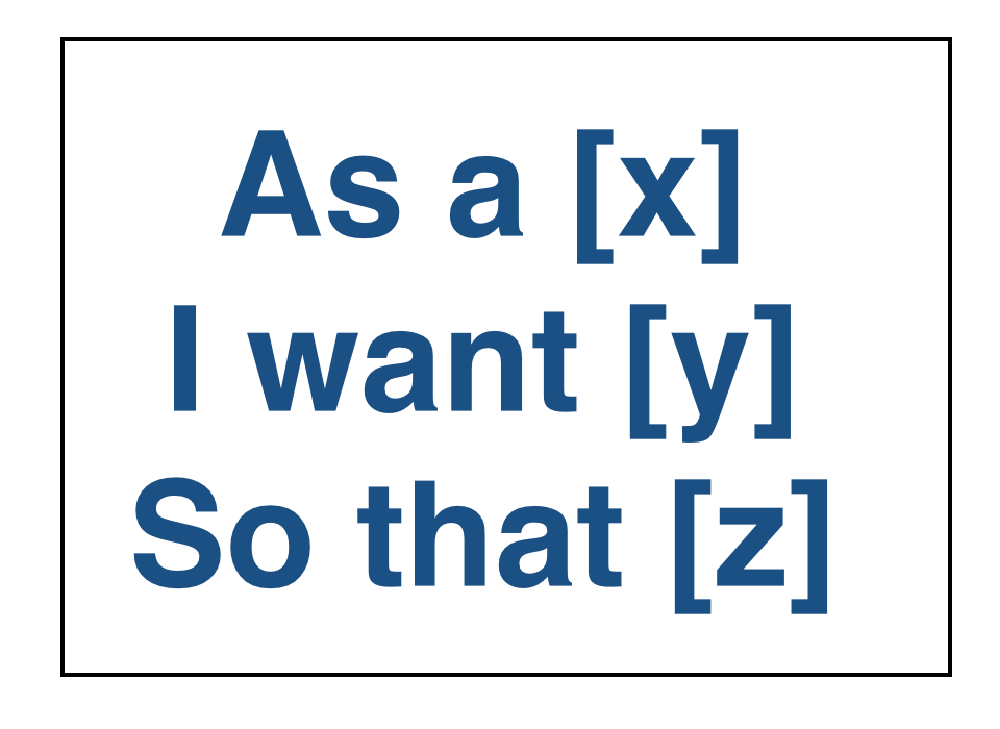
\includegraphics[scale=0.35]{capitulos/literatura/userStory.eps}
	\caption{Modelo da estrutura de uma estória do usuário}
	\label{fig:iceCreamConAntiPattern}
\end{figure}

Onde Y é o comportamento ou funcionalidade esperada, Z é o benefício ou valor desta característica e X é o papel ou pessoa beneficiada com essa funcionalidade. Para ilustrar um exemplo de como a estória do usuário pode ser escrita, temos:

\begin{figure}[H]
	\centering
	\captionsetup{justification=centering,margin=2cm}
	\includegraphics[scale=0.35]{capitulos/literatura/exemploUserStory.eps}
	\caption{Exemplo de escrita de uma estória do usuário}
	\label{fig:iceCreamConAntiPattern}
\end{figure}
	
O título da estória descreve a atividade que é realizada por um usuário em um determinado papel. A funcionalidade desejada fornecida pelo usuário, específica a característica que o sistema deve possuir , com a implementação desta funcionalidade o usuário obtém um benefício. Utilizando este modelo fica clara a necessidade de implementação de tal característica e o seu impacto para o usuário. Os desenvolvedores sabem como o sistema deve se comportar e com quem devem falar sobre tal requisito. Além disso, os usuários entram em questionamento sobre a real necessidade de tal característica, uma vez que é perguntado qual ganho ele terá com essa implementação.


Um cenário descreve a forma como o sistema  deve se comportar quando está em um estado específico e um evento acontece, para que a funcionalidade ou característica requisitada esteja funcionando de acordo com o esperado.  O resultado do cenário altera o estado do sistema ou produz uma saída para o usuário. Nós usamos o termo ação em vez de saída do sistema \cite{Solis2011} porque, uma ação representa qualquer comportamento de reação do sistema.	

\begin{figure}[H]
	\centering
	\captionsetup{justification=centering,margin=2cm}
	\includegraphics[scale=0.35]{capitulos/literatura/modeloCenario.eps}
	\caption{Exemplo de modelo da estrutura de um cenário}
	\label{fig:iceCreamConAntiPattern}
\end{figure}	
	
	\item Automação de testes de aceitação com regras de mapeamento

Testes de aceitação com BDD é uma especificação do comportamento do sistema, especificação executável que verifica as interações (conduta) dos objetos em vezes de só avaliar seus estados \cite{bddIntroducing}. Um cenário é composto de várias etapas, a etapa é uma abstração que representa um dos elementos do cenário que são: contexto, eventos e ações. Um exemplo do significado deles pode ser: em um caso particular de uma estória do usuário ou contexto C, quando um evento X acontece, a resposta do sistema deve ser Z. Cada passo desse é mapeado para um método de teste da aplicação. Para que um cenário passe (seja validado), é necessário que todas as suas etapas também passem, estas etapas são normalmente chamadas de "steps". A principal ideia no uso do BDD é o foco em prevenir falhas de comunicação, o que significa que todos no time estão se comunicando de maneira mais frequente, eficaz e com base em exemplos reais, não se baseando em abstrações ou em requisitos imperativos. 

Para a implementação da automação dos testes deste trabalho, foram escritos alguns cenários para demonstrar como pode ser utilizado na prática de desenvolvimento e testes com BDD (Behaviour Driven Development) usando a ferramenta Cucumber, que será explicado na próxima sessão.
\end{itemize}

\subsection{Cucumber}

Existem diversas ferramentas que possibilita a aplicação do BDD, mas para este trabalho vamos nos ater a uma delas, o Cucumber. Na utilização do Cucumber, as funcionalidades do sistema são escritas em arquivos de texto e em uma linguagem de domínio específico chamada Gherkin \cite{gherkin}, muito parecida com a linguagem natural, mas que contém algumas palavras chaves \cite{Cucumber}.  Para entender a estrutura básica que o Cucumber define para as estórias do usuário, a seguir são listados alguns conceitos.

\begin{itemize}

	\item Para o Cucumber, todas as  estórias do usuário referentes a uma funcionalidade do sistema estarão agrupadas em um arquivo com a extensão ".feature";
	\item No início de cada arquivo existe um resumo da funcionalidade com um formato bem simples: um título, qual o problema a ser resolvido, qual ator trabalha nesta história e qual o resultado desejado;
	\item Logo depois são definidos os cenários, que é estória propriamente dita ou critérios de aceitação que validam a estória, cada arquivo tem pelo menos um cenário;
	\item Cada história ou cenário é composto por uma descrição ou título, uma ou mais pré-condições, uma ou mais ações e uma ou mais verificações.
\end{itemize}

Essa é a estrutura básica de um arquivo ".fature" do Cucumber, esta definição pode ser genérica e gerar dúvidas, então para maior entendimento vamos especificar melhor como é essa estrutura e seu funcionamento. Os testes utilizando BDD são compostos, basicamente, por arquivos que especificam as funcionalidades ".feature" como mencionado e por arquivos de definição de passos "steps". Os arquivos com as funcionalidades são compostos por cenários, que exemplificam uma ou mais regras de negócio de como o sistema deve se comportar.

\begin{figure}[H]
	\centering
	\captionsetup{justification=centering,margin=2cm}
	\includegraphics[scale=0.35]{capitulos/literatura/exemoloCenario.eps}
	\caption{Ilustração de um cenário no arquivo .feature}
	\label{fig:iceCreamConAntiPattern}
\end{figure}	

Afim de aplicar alguns cenários na automação dos testes desenvolvidos neste trabalho, foi utilizado o Cucucmber-JVM [33] que da suporte a implementação do Cucumber na linguagem de programação Java.
